\documentclass[a4paper]{article}

\usepackage{placeins}
\usepackage{newclude}
\usepackage{lmodern}
\usepackage{amssymb,amsmath}
\usepackage{ifxetex,ifluatex}
\usepackage{fixltx2e} % provides \textsubscript
\ifnum 0\ifxetex 1\fi\ifluatex 1\fi=0 % if pdftex
\usepackage[T1]{fontenc}
\usepackage[utf8]{inputenc}
\else % if luatex or xelatex
\ifxetex
\usepackage{mathspec}
\else
\usepackage{fontspec}
\fi
\defaultfontfeatures{Ligatures=TeX,Scale=MatchLowercase}
\fi
% use upquote if available, for straight quotes in verbatim environments
\IfFileExists{upquote.sty}{\usepackage{upquote}}{}
% use microtype if available
\IfFileExists{microtype.sty}{%
	\usepackage{microtype}
	\UseMicrotypeSet[protrusion]{basicmath} % disable protrusion for tt fonts
}{}
\usepackage[margin=1in]{geometry}
\usepackage{hyperref}
\hypersetup{unicode=true,
	pdftitle={lab1},
	pdfborder={0 0 0},
	breaklinks=true}
\urlstyle{same}  % don't use monospace font for urls
\usepackage{color}
\usepackage{fancyvrb}
\newcommand{\VerbBar}{|}
\newcommand{\VERB}{\Verb[commandchars=\\\{\}]}
\DefineVerbatimEnvironment{Highlighting}{Verbatim}{commandchars=\\\{\}}
% Add ',fontsize=\small' for more characters per line
\usepackage{framed}
\definecolor{shadecolor}{RGB}{248,248,248}
\newenvironment{Shaded}{\begin{snugshade}}{\end{snugshade}}
\newcommand{\KeywordTok}[1]{\textcolor[rgb]{0.13,0.29,0.53}{\textbf{{#1}}}}
\newcommand{\DataTypeTok}[1]{\textcolor[rgb]{0.13,0.29,0.53}{{#1}}}
\newcommand{\DecValTok}[1]{\textcolor[rgb]{0.00,0.00,0.81}{{#1}}}
\newcommand{\BaseNTok}[1]{\textcolor[rgb]{0.00,0.00,0.81}{{#1}}}
\newcommand{\FloatTok}[1]{\textcolor[rgb]{0.00,0.00,0.81}{{#1}}}
\newcommand{\ConstantTok}[1]{\textcolor[rgb]{0.00,0.00,0.00}{{#1}}}
\newcommand{\CharTok}[1]{\textcolor[rgb]{0.31,0.60,0.02}{{#1}}}
\newcommand{\SpecialCharTok}[1]{\textcolor[rgb]{0.00,0.00,0.00}{{#1}}}
\newcommand{\StringTok}[1]{\textcolor[rgb]{0.31,0.60,0.02}{{#1}}}
\newcommand{\VerbatimStringTok}[1]{\textcolor[rgb]{0.31,0.60,0.02}{{#1}}}
\newcommand{\SpecialStringTok}[1]{\textcolor[rgb]{0.31,0.60,0.02}{{#1}}}
\newcommand{\ImportTok}[1]{{#1}}
\newcommand{\CommentTok}[1]{\textcolor[rgb]{0.56,0.35,0.01}{\textit{{#1}}}}
\newcommand{\DocumentationTok}[1]{\textcolor[rgb]{0.56,0.35,0.01}{\textbf{\textit{{#1}}}}}
\newcommand{\AnnotationTok}[1]{\textcolor[rgb]{0.56,0.35,0.01}{\textbf{\textit{{#1}}}}}
\newcommand{\CommentVarTok}[1]{\textcolor[rgb]{0.56,0.35,0.01}{\textbf{\textit{{#1}}}}}
\newcommand{\OtherTok}[1]{\textcolor[rgb]{0.56,0.35,0.01}{{#1}}}
\newcommand{\FunctionTok}[1]{\textcolor[rgb]{0.00,0.00,0.00}{{#1}}}
\newcommand{\VariableTok}[1]{\textcolor[rgb]{0.00,0.00,0.00}{{#1}}}
\newcommand{\ControlFlowTok}[1]{\textcolor[rgb]{0.13,0.29,0.53}{\textbf{{#1}}}}
\newcommand{\OperatorTok}[1]{\textcolor[rgb]{0.81,0.36,0.00}{\textbf{{#1}}}}
\newcommand{\BuiltInTok}[1]{{#1}}
\newcommand{\ExtensionTok}[1]{{#1}}
\newcommand{\PreprocessorTok}[1]{\textcolor[rgb]{0.56,0.35,0.01}{\textit{{#1}}}}
\newcommand{\AttributeTok}[1]{\textcolor[rgb]{0.77,0.63,0.00}{{#1}}}
\newcommand{\RegionMarkerTok}[1]{{#1}}
\newcommand{\InformationTok}[1]{\textcolor[rgb]{0.56,0.35,0.01}{\textbf{\textit{{#1}}}}}
\newcommand{\WarningTok}[1]{\textcolor[rgb]{0.56,0.35,0.01}{\textbf{\textit{{#1}}}}}
\newcommand{\AlertTok}[1]{\textcolor[rgb]{0.94,0.16,0.16}{{#1}}}
\newcommand{\ErrorTok}[1]{\textcolor[rgb]{0.64,0.00,0.00}{\textbf{{#1}}}}
\newcommand{\NormalTok}[1]{{#1}}
\usepackage{graphicx,grffile}
\makeatletter
\def\maxwidth{\ifdim\Gin@nat@width>\linewidth\linewidth\else\Gin@nat@width\fi}
\def\maxheight{\ifdim\Gin@nat@height>\textheight\textheight\else\Gin@nat@height\fi}
\makeatother
% Scale images if necessary, so that they will not overflow the page
% margins by default, and it is still possible to overwrite the defaults
% using explicit options in \includegraphics[width, height, ...]{}
\setkeys{Gin}{width=\maxwidth,height=\maxheight,keepaspectratio}
\IfFileExists{parskip.sty}{%
	\usepackage{parskip}
}{% else
\setlength{\parindent}{0pt}
\setlength{\parskip}{6pt plus 2pt minus 1pt}
}
\setlength{\emergencystretch}{3em}  % prevent overfull lines
\providecommand{\tightlist}{%
	\setlength{\itemsep}{0pt}\setlength{\parskip}{0pt}}
\setcounter{secnumdepth}{3} %numbering!!!!
\setcounter{tocdepth}{3}
% Redefines (sub)paragraphs to behave more like sections
\ifx\paragraph\undefined\else
\let\oldparagraph\paragraph
\renewcommand{\paragraph}[1]{\oldparagraph{#1}\mbox{}}
\fi
\ifx\subparagraph\undefined\else
\let\oldsubparagraph\subparagraph
\renewcommand{\subparagraph}[1]{\oldsubparagraph{#1}\mbox{}}
\fi

\usepackage[english, polish]{babel}
\usepackage[utf8]{inputenc}
\usepackage{amsmath}
\usepackage{graphicx}
\usepackage[colorinlistoftodos]{todonotes}

\usepackage{fancyhdr}% http://ctan.org/pkg/fancyhdr

\fancyhf{}% Clear all headers/footers
\renewcommand{\headrulewidth}{0pt}% No header rule
\renewcommand{\footrulewidth}{0pt}% No footer rule
\fancyfoot[C]{\thepage}%


\fancypagestyle{firstpage}{
    \fancyfoot[C]{
    Prowadzący: mgr inż. Marcin Stasiak
    }
    }

\title{\normalsize \textsc{
        \Large{POLITECHNIKA POZNAŃSKA}\\
		\large{Wydział Elektryczny}\\
		\normalsize
		Instytut Matematyki\\
		Zakład Zastosowań Matematyki
		}
    \\[4.0cm]
    \Large{Praca semestralna}\\
    [0.5cm]
    \Huge{Metoda Różnic Skończonych}
    \normalsize \vspace*{5\baselineskip}
    }
\author{Mateusz Talarski\\i\\Piotr Wyrwiński}

\date{}
\begin{document}
	\maketitle
    \thispagestyle{firstpage}
	\newpage
	
	\tableofcontents
	\newpage
	
	
    %	\section{Macierze Kroneckera}
	\subsection{Iloczyn Kroneckera}	
		
		Jeżeli \textbf{A} jest macierzą o wymiarze $m \times n$, oraz \textbf{B} jest $p \times q$, to \textbf{iloczynem Kroneckera (iloczynem tensorowym)} $\mathbf{A \otimes B}$ nazywamy macierz blokową $mp \times nq$
		
	$$\mathbf{A \otimes B} = \begin{bmatrix} a_{11} \mathbf{B} & \cdots & a_{1n}\mathbf{B} \\ \vdots & \ddots & \vdots \\ a_{m1} \mathbf{B} & \cdots & a_{mn} \mathbf{B} \end{bmatrix}$$
	
	Z definicji tej wynika, że mnożone macierze \textbf{A} i \textbf{B} mogą być dowolnych rozmiarów.
	
	W ogólności $\mathbf{A \otimes B} \neq \mathbf{B \otimes A}$.
	
		\textbf{Przykład}
	$$\begin{bmatrix}1&2\\3&4\\\end{bmatrix}\otimes {\begin{bmatrix}0&5\\6&7\\\end{bmatrix}}={\begin{bmatrix}1\cdot {\begin{bmatrix}0&5\\6&7\\\end{bmatrix}}&2\cdot {\begin{bmatrix}0&5\\6&7\\\end{bmatrix}}\\3\cdot {\begin{bmatrix}0&5\\6&7\\\end{bmatrix}}&4\cdot {\begin{bmatrix}0&5\\6&7\\\end{bmatrix}}\\\end{bmatrix}}={\begin{bmatrix}1\cdot 0&1\cdot 5&2\cdot 0&2\cdot 5\\1\cdot 6&1\cdot 7&2\cdot 6&2\cdot 7\\3\cdot 0&3\cdot 5&4\cdot 0&4\cdot 5\\3\cdot 6&3\cdot 7&4\cdot 6&4\cdot 7\\\end{bmatrix}}={\begin{bmatrix}0&5&0&10\\6&7&12&14\\0&15&0&20\\18&21&24&28\end{bmatrix}}$$
	
	\subsection{Cel ćwiczenia}
	Dla zadanych macierzy A, B, C mieliśmy utworzyć odpowienie macierze przy pomocy iloczynu Kroneckera.
	
		$$A = \begin{bmatrix}2&-1\\-1&2\\\end{bmatrix},  B = \begin{bmatrix}0&-1\\2&3\\\end{bmatrix},  C = \begin{bmatrix}1&1\\1&2\\\end{bmatrix} $$
		
	Przykłady zostały wykonane dla rzędów macierzy n = 6
		
\begin{samepage}
\begin{Shaded}
\begin{Highlighting}[]
\FunctionTok{clc}\NormalTok{,}\FunctionTok{clear}\NormalTok{;}
        
\NormalTok{A=[}\FloatTok{2}\NormalTok{, -}\FloatTok{1}\NormalTok{;-}\FloatTok{1}\NormalTok{,}\FloatTok{2}\NormalTok{];}
\NormalTok{B=[}\FloatTok{0}\NormalTok{,-}\FloatTok{1}\NormalTok{;}\FloatTok{2}\NormalTok{,}\FloatTok{3}\NormalTok{];}
\NormalTok{C=[}\FloatTok{1}\NormalTok{,}\FloatTok{1}\NormalTok{;}\FloatTok{1}\NormalTok{,}\FloatTok{2}\NormalTok{];}
        
\NormalTok{n=}\FloatTok{input("Enter a number: ")}\NormalTok{;}
        
\NormalTok{E1 = }\FunctionTok{kron}\NormalTok{(}\FunctionTok{eye}\NormalTok{(n),A)}
\end{Highlighting}
\end{Shaded}
\end{samepage}
\begin{samepage}
\begin{verbatim}
## E1 =
## 
##    2  -1   0   0   0   0   0   0   0   0   0   0
##   -1   2   0   0   0   0   0   0   0   0   0   0
##    0   0   2  -1   0   0   0   0   0   0   0   0
##    0   0  -1   2   0   0   0   0   0   0   0   0
##    0   0   0   0   2  -1   0   0   0   0   0   0
##    0   0   0   0  -1   2   0   0   0   0   0   0
##    0   0   0   0   0   0   2  -1   0   0   0   0
##    0   0   0   0   0   0  -1   2   0   0   0   0
##    0   0   0   0   0   0   0   0   2  -1   0   0
##    0   0   0   0   0   0   0   0  -1   2   0   0
##    0   0   0   0   0   0   0   0   0   0   2  -1
##    0   0   0   0   0   0   0   0   0   0  -1   2
\end{verbatim}
\end{samepage}

\begin{samepage}
\begin{Shaded}
	\begin{Highlighting}[]
\NormalTok{E2 = }\FunctionTok{kron}\NormalTok{(}\FunctionTok{diag}\NormalTok{(v),A)}
	\end{Highlighting}
\end{Shaded}
\end{samepage}

\begin{samepage}
\begin{verbatim}
## E2 =
## 
##    2  -1   0   0   0   0   0   0   0   0   0   0
##   -1   2   0   0   0   0   0   0   0   0   0   0
##    0   0   4  -2   0   0   0   0   0   0   0   0
##    0   0  -2   4   0   0   0   0   0   0   0   0
##    0   0   0   0   4  -2   0   0   0   0   0   0
##    0   0   0   0  -2   4   0   0   0   0   0   0
##    0   0   0   0   0   0   4  -2   0   0   0   0
##    0   0   0   0   0   0  -2   4   0   0   0   0
##    0   0   0   0   0   0   0   0   4  -2   0   0
##    0   0   0   0   0   0   0   0  -2   4   0   0
##    0   0   0   0   0   0   0   0   0   0   2  -1
##    0   0   0   0   0   0   0   0   0   0  -1   2
\end{verbatim}          
\end{samepage}

\begin{samepage}
\begin{Shaded}
	\begin{Highlighting}[]

\NormalTok{v = [}\FloatTok{1}\NormalTok{;-}\FloatTok{1}\NormalTok{*}\FunctionTok{diag}\NormalTok{(}\FunctionTok{eye}\NormalTok{(n-}\FloatTok{2}\NormalTok{));}\FloatTok{1}\NormalTok{];}
	
\NormalTok{E3 = }\FunctionTok{kron}\NormalTok{(}\FunctionTok{diag}\NormalTok{(v),A) +\textbackslash{}}
\FunctionTok{kron}\NormalTok{(}\FunctionTok{diag}\NormalTok{(}\FunctionTok{diag}\NormalTok{(}\FunctionTok{eye}\NormalTok{(n-}\FloatTok{1}\NormalTok{)),}\FloatTok{1}\NormalTok{),B) +\textbackslash{}}
\FunctionTok{kron}\NormalTok{(}\FunctionTok{diag}\NormalTok{(}\FunctionTok{diag}\NormalTok{(}\FunctionTok{eye}\NormalTok{(n-}\FloatTok{1}\NormalTok{)),-}\FloatTok{1}\NormalTok{),B);}
	\end{Highlighting}
\end{Shaded}                                        
\end{samepage}
                    
\begin{samepage}
\begin{verbatim} 
## E3 =
## 
##    2  -1   0  -1   0   0   0   0   0   0   0   0
##   -1   2   2   3   0   0   0   0   0   0   0   0
##    0  -1  -2   1   0  -1   0   0   0   0   0   0
##    2   3   1  -2   2   3   0   0   0   0   0   0
##    0   0   0  -1  -2   1   0  -1   0   0   0   0
##    0   0   2   3   1  -2   2   3   0   0   0   0
##    0   0   0   0   0  -1  -2   1   0  -1   0   0
##    0   0   0   0   2   3   1  -2   2   3   0   0
##    0   0   0   0   0   0   0  -1  -2   1   0  -1
##    0   0   0   0   0   0   2   3   1  -2   2   3
##    0   0   0   0   0   0   0   0   0  -1   2  -1
##    0   0   0   0   0   0   0   0   2   3  -1   2
\end{verbatim}
\end{samepage}

\begin{samepage}
\begin{Shaded}
	\begin{Highlighting}[]
\NormalTok{v = [}\FloatTok{1}\NormalTok{;}\FloatTok{2}\NormalTok{*}\FunctionTok{diag}\NormalTok{(}\FunctionTok{eye}\NormalTok{(n-}\FloatTok{2}\NormalTok{));}\FloatTok{1}\NormalTok{];}

\NormalTok{E4 = }\FunctionTok{kron}\NormalTok{(}\FunctionTok{diag}\NormalTok{(v),A) +\textbackslash{}}
\FunctionTok{kron}\NormalTok{(}\FunctionTok{diag}\NormalTok{(}\FunctionTok{diag}\NormalTok{(}\FunctionTok{eye}\NormalTok{(n-}\FloatTok{1}\NormalTok{)),}\FloatTok{1}\NormalTok{),B) +\textbackslash{}}
\FunctionTok{kron}\NormalTok{(}\FunctionTok{diag}\NormalTok{(}\FunctionTok{diag}\NormalTok{(}\FunctionTok{eye}\NormalTok{(n-}\FloatTok{1}\NormalTok{)),-}\FloatTok{1}\NormalTok{),B');}		
	\end{Highlighting}
\end{Shaded}
\end{samepage}

\begin{samepage}
\begin{verbatim}
## E4 =
## 
##    2  -1   0  -1   0   0   0   0   0   0   0   0
##   -1   2   2   3   0   0   0   0   0   0   0   0
##    0   2   4  -2   0  -1   0   0   0   0   0   0
##   -1   3  -2   4   2   3   0   0   0   0   0   0
##    0   0   0   2   4  -2   0  -1   0   0   0   0
##    0   0  -1   3  -2   4   2   3   0   0   0   0
##    0   0   0   0   0   2   4  -2   0  -1   0   0
##    0   0   0   0  -1   3  -2   4   2   3   0   0
##    0   0   0   0   0   0   0   2   4  -2   0  -1
##    0   0   0   0   0   0  -1   3  -2   4   2   3
##    0   0   0   0   0   0   0   0   0   2   2  -1
##    0   0   0   0   0   0   0   0  -1   3  -1   2
\end{verbatim}
\end{samepage}

\begin{samepage}
\begin{Shaded}
	\begin{Highlighting}[]
\NormalTok{E5=}\FunctionTok{kron}\NormalTok{(}\FunctionTok{eye}\NormalTok{(n),A) +\textbackslash{}}
\FunctionTok{kron}\NormalTok{(}\FunctionTok{diag}\NormalTok{(}\FunctionTok{diag}\NormalTok{(}\FunctionTok{eye}\NormalTok{(n-}\FloatTok{2}\NormalTok{)),}\FloatTok{2}\NormalTok{),B') +\textbackslash{}}
\FunctionTok{kron}\NormalTok{(}\FunctionTok{diag}\NormalTok{(}\FunctionTok{diag}\NormalTok{(}\FunctionTok{eye}\NormalTok{(n-}\FloatTok{2}\NormalTok{)),-}\FloatTok{2}\NormalTok{),B);}		
	\end{Highlighting}
\end{Shaded}
\end{samepage}

\begin{samepage}
\begin{verbatim}
## E5 =
## 
##    2  -1   0   0   0   2   0   0   0   0   0   0
##   -1   2   0   0  -1   3   0   0   0   0   0   0
##    0   0   2  -1   0   0   0   2   0   0   0   0
##    0   0  -1   2   0   0  -1   3   0   0   0   0
##    0  -1   0   0   2  -1   0   0   0   2   0   0
##    2   3   0   0  -1   2   0   0  -1   3   0   0
##    0   0   0  -1   0   0   2  -1   0   0   0   2
##    0   0   2   3   0   0  -1   2   0   0  -1   3
##    0   0   0   0   0  -1   0   0   2  -1   0   0
##    0   0   0   0   2   3   0   0  -1   2   0   0
##    0   0   0   0   0   0   0  -1   0   0   2  -1
##    0   0   0   0   0   0   2   3   0   0  -1   2
\end{verbatim}
\end{samepage}

\begin{samepage}
\begin{Shaded}
	\begin{Highlighting}[]
\NormalTok{v = [}\FloatTok{1}\NormalTok{;}\FunctionTok{zeros}\NormalTok{(n-}\FloatTok{2}\NormalTok{,}\FloatTok{1}\NormalTok{);}\FloatTok{1}\NormalTok{];}
\NormalTok{v1 = [}\FloatTok{0}\NormalTok{;}\FunctionTok{diag}\NormalTok{(}\FunctionTok{eye}\NormalTok{(n-}\FloatTok{2}\NormalTok{));}\FloatTok{0}\NormalTok{];}

\NormalTok{E6 = }\FunctionTok{kron}\NormalTok{(}\FunctionTok{diag}\NormalTok{(v),C)+ }\FunctionTok{kron}\NormalTok{(}\FunctionTok{diag}\NormalTok{(v1),A) +\textbackslash{}}
\FunctionTok{kron}\NormalTok{(}\FunctionTok{diag}\NormalTok{(}\FunctionTok{diag}\NormalTok{(}\FunctionTok{eye}\NormalTok{(n-}\FloatTok{2}\NormalTok{)),}\FloatTok{2}\NormalTok{),}\FloatTok{3}\NormalTok{*B') +\textbackslash{}}
\FunctionTok{kron}\NormalTok{(}\FunctionTok{diag}\NormalTok{(}\FunctionTok{diag}\NormalTok{(}\FunctionTok{eye}\NormalTok{(n-}\FloatTok{2}\NormalTok{)),-}\FloatTok{2}\NormalTok{),}\FloatTok{2}\NormalTok{*B) +\textbackslash{}}
\NormalTok{flip(}\FunctionTok{kron}\NormalTok{(}\FunctionTok{diag}\NormalTok{(v), flip(}\FunctionTok{eye}\NormalTok{(}\FloatTok{2}\NormalTok{))));}		
	\end{Highlighting}
\end{Shaded}
\end{samepage}

\begin{samepage}
\begin{verbatim}
## E6 =
## 
##    1   1   0   0   0   6   0   0   0   0   1   0
##    1   2   0   0  -3   9   0   0   0   0   0   1
##    0   0   2  -1   0   0   0   6   0   0   0   0
##    0   0  -1   2   0   0  -3   9   0   0   0   0
##    0  -2   0   0   2  -1   0   0   0   6   0   0
##    4   6   0   0  -1   2   0   0  -3   9   0   0
##    0   0   0  -2   0   0   2  -1   0   0   0   6
##    0   0   4   6   0   0  -1   2   0   0  -3   9
##    0   0   0   0   0  -2   0   0   2  -1   0   0
##    0   0   0   0   4   6   0   0  -1   2   0   0
##    1   0   0   0   0   0   0  -2   0   0   1   1
##    0   1   0   0   0   0   4   6   0   0   1   2
\end{verbatim}
\end{samepage}

\begin{samepage}
\begin{Shaded}
	\begin{Highlighting}[]
\NormalTok{v=[}\FloatTok{1}\NormalTok{;}\FunctionTok{zeros}\NormalTok{(n-}\FloatTok{2}\NormalTok{,}\FloatTok{1}\NormalTok{);}\FloatTok{1}\NormalTok{];}
\NormalTok{v1=[}\FloatTok{0}\NormalTok{;}\FloatTok{1}\NormalTok{;}\FunctionTok{zeros}\NormalTok{(n-}\FloatTok{4}\NormalTok{,}\FloatTok{1}\NormalTok{);}\FloatTok{1}\NormalTok{;}\FloatTok{0}\NormalTok{];}
\NormalTok{v2=[}\FloatTok{0}\NormalTok{;}\FloatTok{0}\NormalTok{;}\FloatTok{2}\NormalTok{*}\FunctionTok{diag}\NormalTok{(}\FunctionTok{eye}\NormalTok{(n-}\FloatTok{4}\NormalTok{));}\FloatTok{0}\NormalTok{;}\FloatTok{0}\NormalTok{];}

\NormalTok{E7=}\FunctionTok{kron}\NormalTok{(}\FunctionTok{diag}\NormalTok{(v),A) +\textbackslash{}}
\FunctionTok{kron}\NormalTok{(}\FunctionTok{diag}\NormalTok{(v1),B) +\textbackslash{}}
\FunctionTok{kron}\NormalTok{(}\FunctionTok{diag}\NormalTok{(v2),B) +\textbackslash{}}
\FunctionTok{kron}\NormalTok{(}\FunctionTok{diag}\NormalTok{(}\FunctionTok{diag}\NormalTok{(}\FunctionTok{eye}\NormalTok{(n-}\FloatTok{2}\NormalTok{)),}\FloatTok{2}\NormalTok{),C) +\textbackslash{}}
\FunctionTok{kron}\NormalTok{(}\FunctionTok{diag}\NormalTok{(}\FunctionTok{diag}\NormalTok{(}\FunctionTok{eye}\NormalTok{(n-}\FloatTok{2}\NormalTok{)),-}\FloatTok{2}\NormalTok{),C');}		
	\end{Highlighting}
\end{Shaded}
\end{samepage}

\begin{samepage}
\begin{verbatim}
## E7 =
## 
##    2  -1   0   0   1   1   0   0   0   0   0   0
##   -1   2   0   0   1   2   0   0   0   0   0   0
##    0   0   0  -1   0   0   1   1   0   0   0   0
##    0   0   2   3   0   0   1   2   0   0   0   0
##    1   1   0   0   0  -2   0   0   1   1   0   0
##    1   2   0   0   4   6   0   0   1   2   0   0
##    0   0   1   1   0   0   0  -2   0   0   1   1
##    0   0   1   2   0   0   4   6   0   0   1   2
##    0   0   0   0   1   1   0   0   0  -1   0   0
##    0   0   0   0   1   2   0   0   2   3   0   0
##    0   0   0   0   0   0   1   1   0   0   2  -1
##    0   0   0   0   0   0   1   2   0   0  -1   2
\end{verbatim}
\end{samepage}

\begin{samepage}
\begin{Shaded}
	\begin{Highlighting}[]
\NormalTok{v=[}\FloatTok{1}\NormalTok{;}\FunctionTok{zeros}\NormalTok{(n-}\FloatTok{2}\NormalTok{,}\FloatTok{1}\NormalTok{);}\FloatTok{1}\NormalTok{];}
\NormalTok{v1=[}\FloatTok{0}\NormalTok{;}\FloatTok{2}\NormalTok{;}\FunctionTok{zeros}\NormalTok{(n-}\FloatTok{4}\NormalTok{,}\FloatTok{1}\NormalTok{);}\FloatTok{2}\NormalTok{;}\FloatTok{0}\NormalTok{];}
\NormalTok{v2=[}\FloatTok{0}\NormalTok{;}\FloatTok{0}\NormalTok{;}\FunctionTok{diag}\NormalTok{(}\FunctionTok{eye}\NormalTok{(n-}\FloatTok{4}\NormalTok{));}\FloatTok{0}\NormalTok{;}\FloatTok{0}\NormalTok{];}

\NormalTok{E8=}\FunctionTok{kron}\NormalTok{(}\FunctionTok{diag}\NormalTok{(v),A) +\textbackslash{}}
\FunctionTok{kron}\NormalTok{(}\FunctionTok{diag}\NormalTok{(v1),B) + }\FunctionTok{kron}\NormalTok{(}\FunctionTok{diag}\NormalTok{(v2),C) +\textbackslash{}}
\FunctionTok{kron}\NormalTok{(}\FunctionTok{diag}\NormalTok{(}\FunctionTok{diag}\NormalTok{(}\FunctionTok{eye}\NormalTok{(n-}\FloatTok{2}\NormalTok{)),}\FloatTok{2}\NormalTok{),}\FunctionTok{eye}\NormalTok{(}\FloatTok{2}\NormalTok{)) +\textbackslash{}}
\FunctionTok{kron}\NormalTok{(}\FunctionTok{diag}\NormalTok{(}\FunctionTok{diag}\NormalTok{(}\FunctionTok{eye}\NormalTok{(n-}\FloatTok{2}\NormalTok{)),-}\FloatTok{2}\NormalTok{),}\FunctionTok{eye}\NormalTok{(}\FloatTok{2}\NormalTok{))+\textbackslash{}}
\NormalTok{flip(}\FunctionTok{kron}\NormalTok{(}\FunctionTok{diag}\NormalTok{(v),flip(A)));}		
	\end{Highlighting}
\end{Shaded}
\end{samepage}

\begin{samepage}
\begin{verbatim}
## E8 =
## 
##    2  -1   0   0   1   0   0   0   0   0   2  -1
##   -1   2   0   0   0   1   0   0   0   0  -1   2
##    0   0   0  -2   0   0   1   0   0   0   0   0
##    0   0   4   6   0   0   0   1   0   0   0   0
##    1   0   0   0   1   1   0   0   1   0   0   0
##    0   1   0   0   1   2   0   0   0   1   0   0
##    0   0   1   0   0   0   1   1   0   0   1   0
##    0   0   0   1   0   0   1   2   0   0   0   1
##    0   0   0   0   1   0   0   0   0  -2   0   0
##    0   0   0   0   0   1   0   0   4   6   0   0
##    2  -1   0   0   0   0   1   0   0   0   2  -1
##   -1   2   0   0   0   0   0   1   0   0  -1   2
\end{verbatim}
\end{samepage}
	
	
    %\include*{Lab1/macierze}

    %\section{Szereg Fouriera}
\subsection{Definicja}
Niech funkcja \textbf{f} będzie określona na odcinku $\mathbf{\left[-\frac{T}{2}, \frac{T}{2}\right]}$ poza skończoną liczbą punktów oraz będzie określona poza przedziałem $\mathbf{\left[-\frac{T}{2}, \frac{T}{2}\right]}${\tiny } poprzez równość $\mathbf{f(x) = f(x + T)}$ (okresowość)
\\ \\
\textbf{Trygonometrycznym szeregiem Fouriera} funkcji f nazywamy szereg funkcyjny następującej postaci:
$$S(x) = \frac{a_{0}}{2} + \sum_{n=1}^{\infty} \left(a_{n} cos\left(\frac{2n\pi}{T} x\right) + b_{n} sin\left(\frac{2n\pi}{T} x\right) \right)$$
O współczynnikach określonych następującymi wzorami:
$$ a_{n} = \frac{2}{T} \int_{-\frac{T}{2}}^{\frac{T}{2}} f(x)cos\left(\frac{2n\pi}{T} x \right) dx,	\quad n = 0,1,2,...$$

$$ b_{n} = \frac{2}{T} \int_{-\frac{T}{2}}^{\frac{T}{2}} f(x)sin\left(\frac{2n\pi}{T} x \right) dx,	\quad n = 1,2,3,...$$


\subsection{Cel ćwiczenia}
Zadane funkcje na określonych przedziałach rozwinęliśmy w szereg Fouriera oraz narysowaliśmy ich wykresy dla \textbf{n = 100}.

\begin{itemize}
    \item $f(x) = x, \quad x\in [-1,1]$
    
    \item $f(x) = x^{2}, \quad x\in [0,1]$
    
    \item $f(x) = sin(x), \quad x\in [-\pi,\pi]$
\end{itemize}

\subsection{Algorytm}
\vspace*{0.1cm}
Poniżej został zaprezentowany kod programu w języku Python:\\

\begin{Shaded}
\begin{Highlighting}[]
\ImportTok{import} \NormalTok{numpy }\ImportTok{as} \NormalTok{np}
\ImportTok{import} \NormalTok{matplotlib.pyplot }\ImportTok{as} \NormalTok{plt}
\KeywordTok{def} \NormalTok{series(x):}
    \NormalTok{const }\OperatorTok{=} \DecValTok{2} \OperatorTok{*} \NormalTok{np.pi }\OperatorTok{*} \NormalTok{x }\OperatorTok{/} \NormalTok{T}
    \ControlFlowTok{return} \KeywordTok{lambda} \NormalTok{x: An(n) }\OperatorTok{*} \NormalTok{np.cos(const }\OperatorTok{*} \NormalTok{n) }\OperatorTok{+} \NormalTok{Bn(n) }\OperatorTok{*} \NormalTok{np.sin(const }\OperatorTok{*} \NormalTok{n)}
\KeywordTok{def} \NormalTok{fab1():}
    \ControlFlowTok{return} \KeywordTok{lambda} \NormalTok{n: }\DecValTok{0}\NormalTok{, }\KeywordTok{lambda} \NormalTok{n: (}\OperatorTok{-}\DecValTok{2}\OperatorTok{*}\NormalTok{(}\OperatorTok{-}\DecValTok{1}\NormalTok{)}\OperatorTok{**}\NormalTok{n)}\OperatorTok{/}\NormalTok{(np.pi }\OperatorTok{*} \NormalTok{n)}
\KeywordTok{def} \NormalTok{fab2():}
    \ControlFlowTok{return} \KeywordTok{lambda} \NormalTok{n: }\DecValTok{1}\OperatorTok{/}\NormalTok{(np.pi}\OperatorTok{**}\DecValTok{2} \OperatorTok{*} \NormalTok{n}\OperatorTok{**}\DecValTok{2}\NormalTok{), }\KeywordTok{lambda} \NormalTok{n: }\OperatorTok{-}\DecValTok{1}\OperatorTok{/}\NormalTok{(np.pi }\OperatorTok{*} \NormalTok{n)}
\KeywordTok{def} \NormalTok{fab3():                                                              }
    \ControlFlowTok{return} \KeywordTok{lambda} \NormalTok{n: }\DecValTok{0}\NormalTok{, }\KeywordTok{lambda} \NormalTok{n: }\DecValTok{1} \ControlFlowTok{if} \NormalTok{n}\OperatorTok{==}\DecValTok{1} \ControlFlowTok{else} \DecValTok{0}   
\KeywordTok{def} \NormalTok{fun():}
    \ControlFlowTok{return} \KeywordTok{lambda} \NormalTok{x: x, }\KeywordTok{lambda} \NormalTok{x: x}\OperatorTok{**}\DecValTok{2}\NormalTok{, }\KeywordTok{lambda} \NormalTok{x: np.sin(x)}
\KeywordTok{def} \NormalTok{plotSeries(x, S, fx):}
    \NormalTok{fig }\OperatorTok{=} \NormalTok{plt.figure()}
    \NormalTok{ax }\OperatorTok{=} \NormalTok{fig.add_subplot(}\DecValTok{111}\NormalTok{)}
    \NormalTok{ax.plot(x, S, x, fx(x), }\StringTok{'r--'}\NormalTok{)}
    \NormalTok{plt.show()}
\NormalTok{rng = int(input('Wpisz range: '))}
\NormalTok{A }\OperatorTok{=} \NormalTok{[}\OperatorTok{-}\DecValTok{1}\NormalTok{, }\DecValTok{0}\NormalTok{, }\OperatorTok{-}\NormalTok{np.pi]}
\NormalTok{B }\OperatorTok{=} \NormalTok{[}\DecValTok{1}\NormalTok{, }\DecValTok{1}\NormalTok{, np.pi]}
\NormalTok{A0 }\OperatorTok{=} \NormalTok{[}\DecValTok{0}\NormalTok{, }\DecValTok{2}\OperatorTok{/}\DecValTok{3}\NormalTok{, }\DecValTok{0}\NormalTok{] }
\NormalTok{F }\OperatorTok{=} \NormalTok{\{}\StringTok{"x"} \NormalTok{: [fab1()], }\StringTok{"x^2"} \NormalTok{: [fab2()], }\StringTok{"sin(x)"} \NormalTok{: [fab3()]\}}
\NormalTok{fx }\OperatorTok{=} \NormalTok{[fun()]}
\NormalTok{X }\OperatorTok{=} \NormalTok{[]}
\NormalTok{Tt }\OperatorTok{=} \NormalTok{[]}
\ControlFlowTok{for} \NormalTok{i }\OperatorTok{in} \BuiltInTok{range}\NormalTok{(}\DecValTok{3}\NormalTok{):}
    \NormalTok{X.append(np.linspace(A[i], B[i], num}\OperatorTok{=}\DecValTok{1000}\NormalTok{))}
    \NormalTok{Tt.append(B[i] }\OperatorTok{-} \NormalTok{A[i])}
\NormalTok{X }\OperatorTok{=} \NormalTok{np.array(X)}
\NormalTok{Tt }\OperatorTok{=} \NormalTok{np.array(Tt)}
\ControlFlowTok{for} \NormalTok{inx, (k, v) }\OperatorTok{in} \BuiltInTok{enumerate}\NormalTok{(F.items()):}
    \NormalTok{a }\OperatorTok{=} \NormalTok{A[inx] }
    \NormalTok{b }\OperatorTok{=} \NormalTok{B[inx]}
    \NormalTok{a0 }\OperatorTok{=} \NormalTok{A0[inx]}
    \NormalTok{T }\OperatorTok{=} \NormalTok{Tt[inx] }
    \NormalTok{x }\OperatorTok{=} \NormalTok{X[inx]}
    \NormalTok{An, Bn }\OperatorTok{=} \NormalTok{v[}\DecValTok{0}\NormalTok{][}\DecValTok{0}\NormalTok{], v[}\DecValTok{0}\NormalTok{][}\DecValTok{1}\NormalTok{]}
    \NormalTok{f }\OperatorTok{=} \NormalTok{series(x)}
    \NormalTok{S }\OperatorTok{=} \NormalTok{np.zeros((x.shape))}
    \ControlFlowTok{for} \NormalTok{i }\OperatorTok{in} \BuiltInTok{range}\NormalTok{(}\DecValTok{1}\NormalTok{, rng}\DecValTok{+1}\NormalTok{):}
        \NormalTok{n }\OperatorTok{=} \NormalTok{i}
        \NormalTok{S }\OperatorTok{+=} \NormalTok{f(x)}
    \NormalTok{S }\OperatorTok{+=} \NormalTok{a0}\OperatorTok{/}\DecValTok{2}
    \NormalTok{plotSeries(x,S, fx[}\DecValTok{0}\NormalTok{][inx])}
\end{Highlighting}
\end{Shaded}
\subsection{Wykresy}
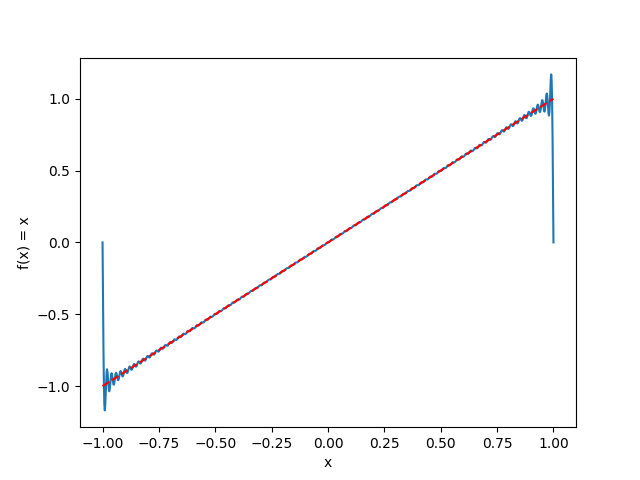
\includegraphics{Lab1/charts/Figure_1.png}

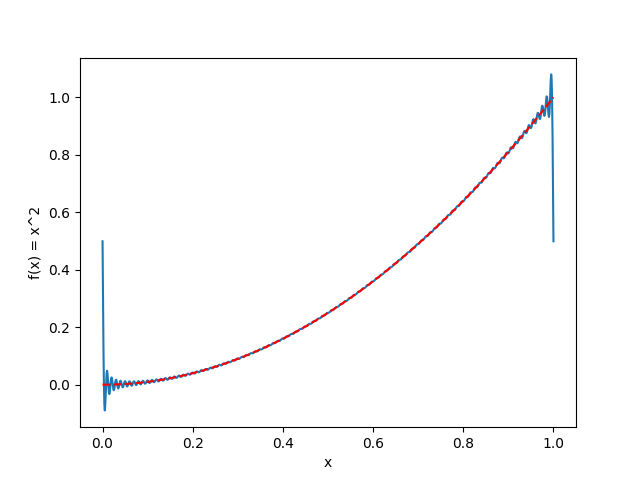
\includegraphics{Lab1/charts/Figure_2.png}
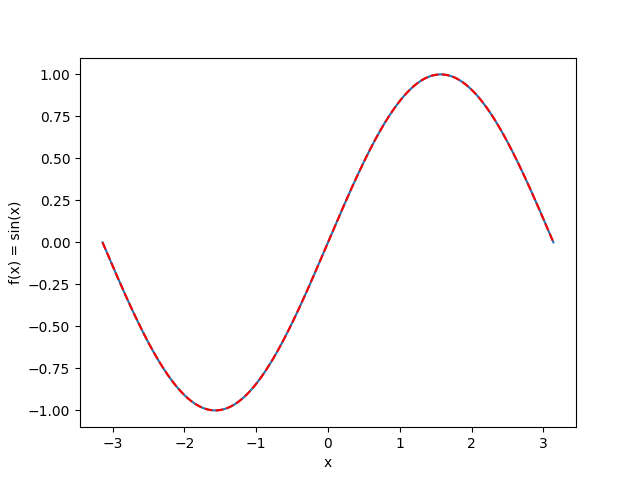
\includegraphics{Lab1/charts/Figure_3.png}

    
    \section{Schematy różnicowe}
\subsection{Definicja}

MRS opiera się na zastąpieniu pochodnych występująych w równaniach różniczkowych poprzez formuły zwane \textbf{schematami różnicowymi}. 

Aproksymacja pochodnej polega na rozwiązywaniu w efektywny sposób równań rózniczkowych zwyczajnych i cząstkowych, gdzie równania te dane są poprzez formuły zawierające nieznaną funkcję, którą chcemy wyznaczyć oraz pochodne dowolnych rzędów, a także stałe i znane funkcje.

Załóżmy, że funkcja $\textbf{f}$ jest różniczkowalna, co oznacza, że pochodna $f'(x_{0})$ jest zdefiniowana i ograniczona w pewnym otoczeniu punktu $x_{0}$.

Wprowadźmy trzy podstawowe schematy różnicowe w celu aproksymacji wartości pochodnej $f'(x_{0})$:

$\bullet$ Schemat \textit{w tył} (backward approximation scheme) 

$$f'(x_{0})\approx D_{-}f(x_{0})=\frac{f(x_{0})-f(x_{0}-h)}{h}$$

$\bullet$ Schemat \textit{w przód} (forward approximation scheme) 

$$f'(x_{0})\approx D_{+}f(x_{0})=\frac{f(x_{0}+h)-f(x_{0})}{h}$$

Obie formuły dają aproksymację rzędu pierwszego, co oznacza, że błąd jest proporcjonalny do wielkości h.

$\bullet$ Schemat \textit{centralny} (central approximation scheme) 

$$f'(x_{0})\approx D_{c}f(x_{0})=\frac{f(x_{0}+h)-f(x_{0}-h)}{2h} = \frac{1}{2}(D_{+}f(x_{0})+D_{-}f(x_{0}))$$

Schemat centralny jest rzędu drugiego, a więc $Error \sim h^{2}$.

	\subsection{Cel ćwiczenia}
Dla wybranej funkcji $f$ mieliśmy użyć schematów różnicowych w celu aproksymacji wartości jej pochodnej, pierwszej oraz drugiej.

Wybraliśmy funkcję $sinus$ w punkcie $x_{0} = 0.3$.

Następnie analitycznie obliczyliśmy pierwszą oraz drugą pochodną w obranym punkcie. Otrzymaliśmy:

$$sin'(0.3)=0.9553$$
$$sin''(0.3)=-0,2955$$

Następnie przystąpiliśmy do obliczeń numerycznych przy wykorzystaniu zaprezentowanych schematów różnicowych.
\newpage

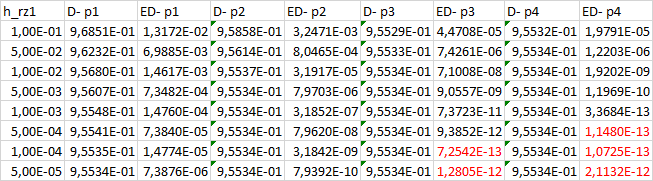
\includegraphics{Lab2/charts/rz1_log_Db_dane.png}

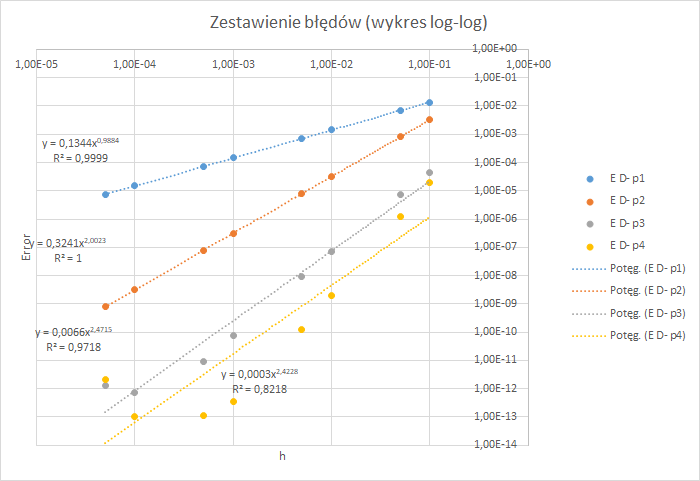
\includegraphics{Lab2/charts/rz1_log_Db.png} 
\newpage


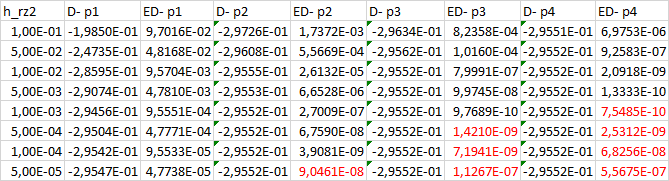
\includegraphics{Lab2/charts/rz2_log_Db_dane.png}

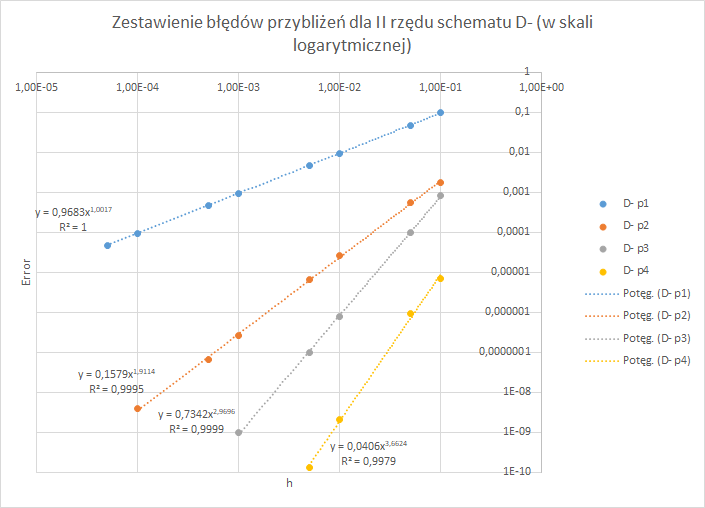
\includegraphics{Lab2/charts/rz2_log_Db.png}
\newpage


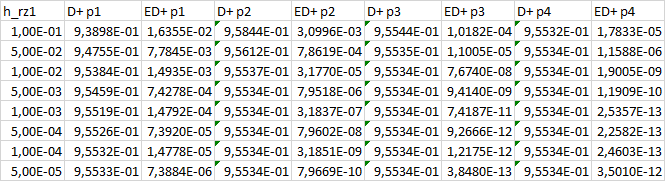
\includegraphics{Lab2/charts/rz1_log_Df_dane.png}

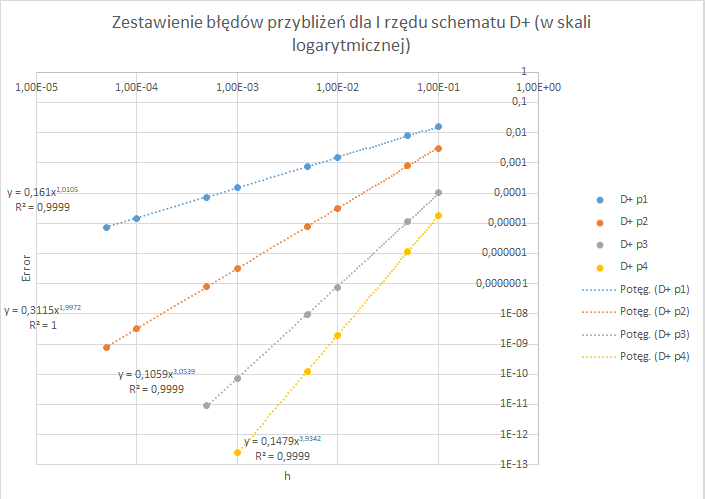
\includegraphics{Lab2/charts/rz1_log_Df.png}
\newpage


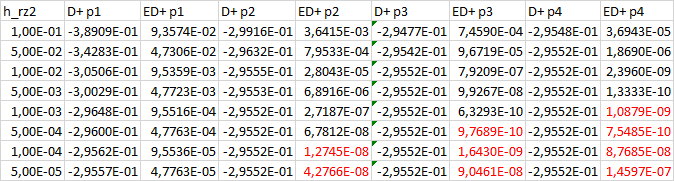
\includegraphics{Lab2/charts/rz2_log_Df_dane.png}

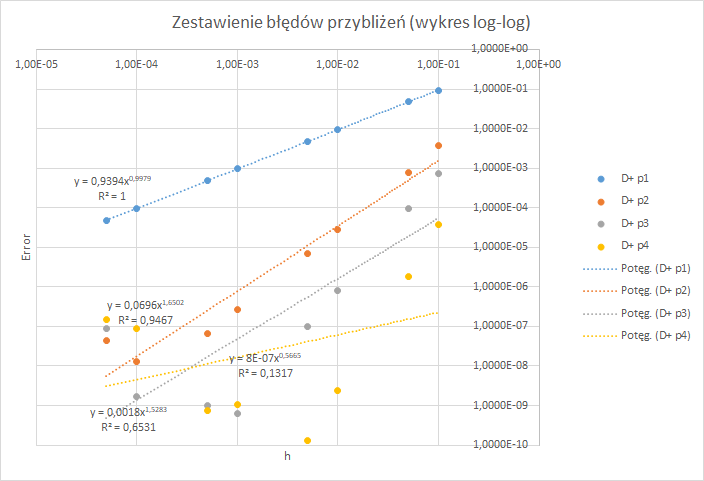
\includegraphics{Lab2/charts/rz2_log_Df.png}
\newpage


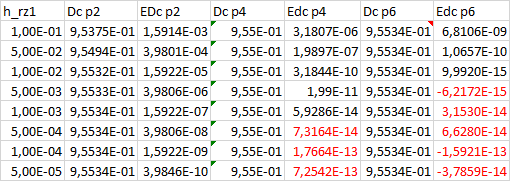
\includegraphics{Lab2/charts/rz1_log_Dc_dane.png}

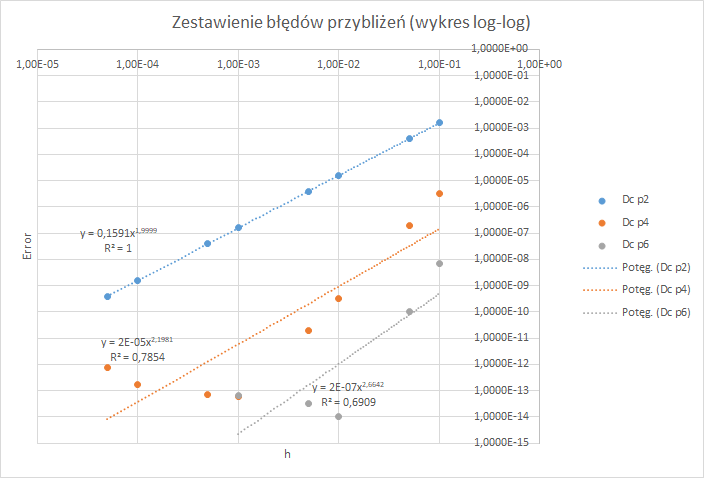
\includegraphics{Lab2/charts/rz1_log_Dc.png}
\newpage


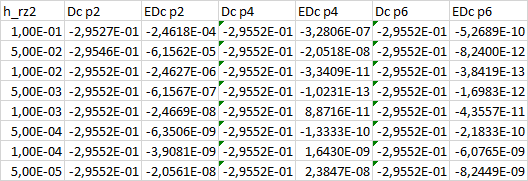
\includegraphics{Lab2/charts/rz2_log_Dc_dane.png}

Zestawienie błędów przybliżeń dla II rzędu schematu Dc na wykresie log-log nie jest możliwe. 

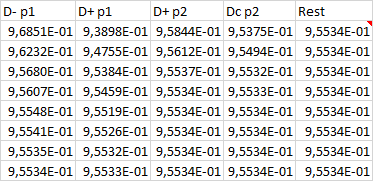
\includegraphics{Lab2/charts/rz1_log_e_dane.png}

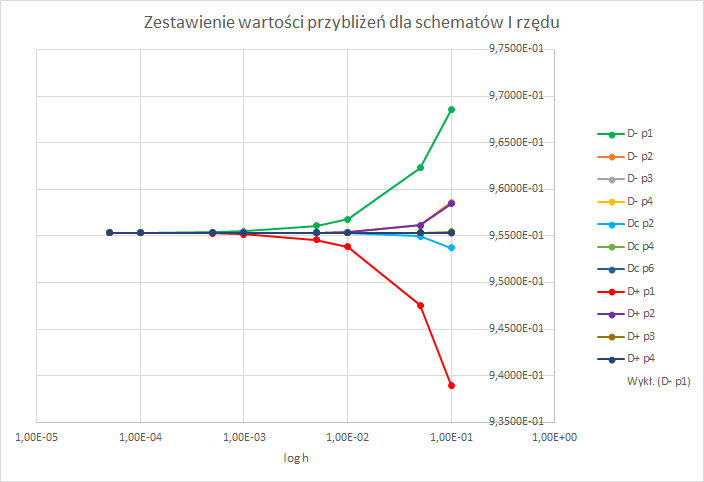
\includegraphics{Lab2/charts/rz1_log_e.png}
\newpage


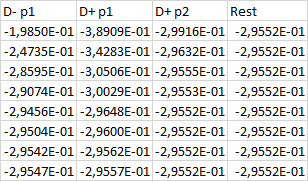
\includegraphics{Lab2/charts/rz2_log_e_dane.png}

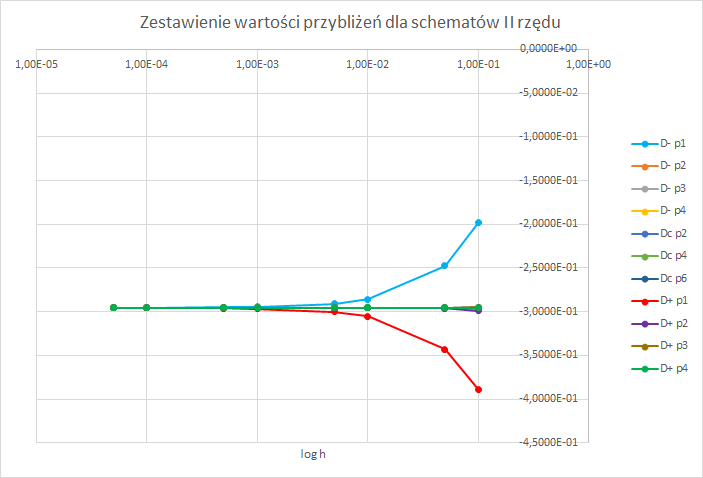
\includegraphics{Lab2/charts/rz2_log_e.png}
\newpage


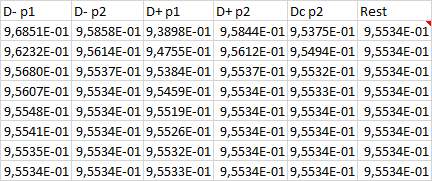
\includegraphics{Lab2/charts/rz1_e_dane.png}

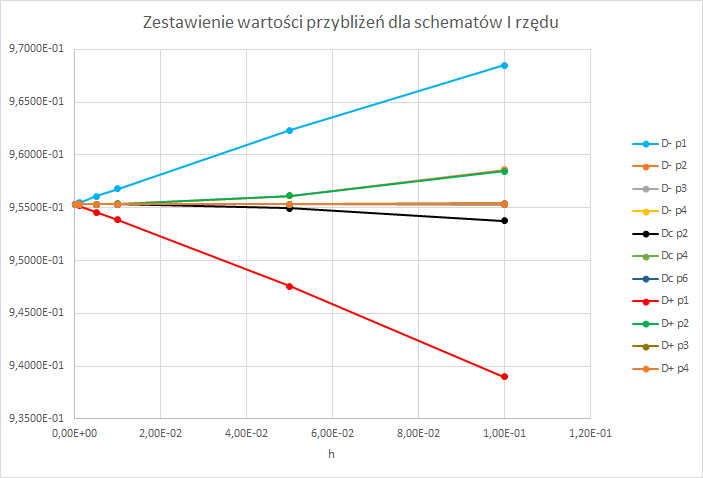
\includegraphics{Lab2/charts/rz1_e.png}
\newpage


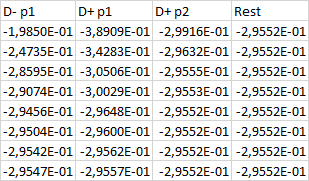
\includegraphics{Lab2/charts/rz2_e_dane.png}

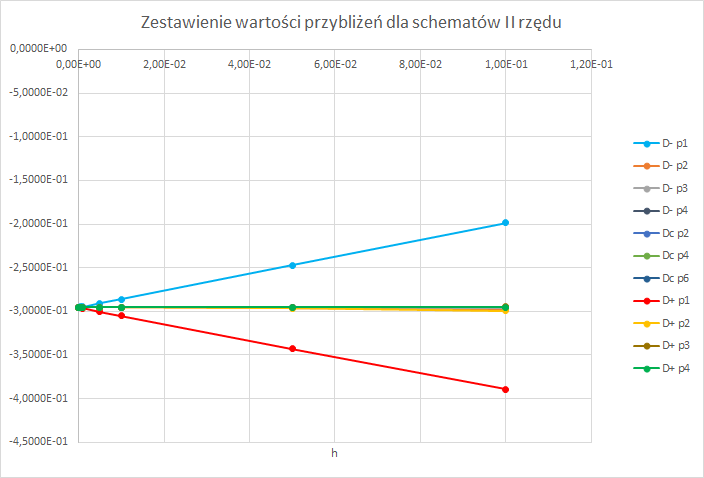
\includegraphics{Lab2/charts/rz2_e.png}




	
\end{document}